\documentclass{cslthse-msc}
\setcounter{tocdepth}{4}
\setcounter{secnumdepth}{4}
\usepackage[utf8]{inputenc}
\usepackage[english]{babel}
\usepackage{amsmath}
\usepackage{amsfonts}
\usepackage{amssymb}
\usepackage{amsthm}
%\usepackage{makeidx}
\usepackage{graphicx}
\usepackage[titletoc, header, page]{appendix}
\usepackage{todo}
\usepackage{float}
\usepackage[hidelinks]{hyperref}
\usepackage{wrapfig}
\usepackage[within=none]{caption}
\usepackage{pdfpages}
\usepackage{svg}
\usepackage{listings}
\usepackage{color}
\newcommand{\hilight}[1]{\colorbox{yellow}{#1}}

\definecolor{mygreen}{rgb}{0,0.6,0}
\definecolor{mygray}{rgb}{0.5,0.5,0.5}
\definecolor{mymauve}{rgb}{0.58,0,0.82}


\lstset{
breaklines=true,
language=SQL,
numbers=left,
numbersep=5pt,
numberstyle=\tiny\color{mygray},
frame=single,
basicstyle=\footnotesize,
captionpos=b
}
\newcommand{\bex}{BeX\textsuperscript{\textregistered}}
\renewcommand{\lstlistingname}{Algorithm}% Listing -> Algorithm
\renewcommand{\lstlistlistingname}{List of \lstlistingname s}% List of Listings -> List of Algorithms



\author{
	Alexander Söderberg \\
	{\normalsize \href{mailto:email@alexandersoderberg.com}{\texttt{email@alexandersoderberg.com}}}
	\and
	Max Åberg \\
    {\normalsize \href{mailto:aaberg.max@gmail.com}{\texttt{aaberg.max@gmail.com}}}
}

\title{Optimizing business intelligence
extraction speed from an
ERP-system’s database}
\subtitle{Master Thesis}
\company{Perfect IT BeX\textsuperscript{\textregistered} AB}
\supervisors{Lennart Söderberg, \href{mailto:lennart@perfectit.se}{\texttt{lennart@perfectit.se}}}{Alma Orucevic Alagic, \href{mailto:alma@cs.lth.se}{\texttt{alma@cs.lth.se}}}
\examiner{Per Andersson, \href{mailto:per.andersson@cs.lth.se}{\texttt{per.andersson@cs.lth.se}}}

\date{\today}

\acknowledgements{
\todo{Skriv acknowledgments}
}

\theabstract{
\todo {Skriv abstract}

}

\keywords{MSc, MsSQL, ERP, Optimization}

%% Only used to display font sizes
\makeatletter
\newcommand\thefontsize[1]{{#1 \f@size pt\par}}
\makeatother
%%%%%%%%%%


\begin{document}
\makefrontmatter
\chapter[Introduction]{Introduction}
2014 was the year of the cloud. Software companies strived to make their services cloud based in order to meet the increasing demands from the market of availability and reliability. 
In today's businesses there's high demand for accurate and up-to-date business intelligence (henceforth referred to as BI).

\chapter{Background}\label{sec:background}

\section{Background}

\section{Problem description}

\section{Thesis Goals} \label{sec:goals}
The goal of this thesis is to examine, test the feasibility and implement a solution for speeding up the generation of BI reports in Perfect IT \bex AB's product \bex Online. To be able to speed up the BI report generation an optimization needs to be done. The optimization needs to be versatile to handle the current system, to handle new functionality and also future company growth. Hence, the optimization needs to be scalable. Taking in to account that Perfect IT \bex has one physical server, the scalability should be vertically \cite{scalability} since the company will provide the system to more clients in the future.\\\\
In order to make the above optimization possible, the following goals have been established:
\begin{enumerate}
\item Acquire knowledge about database optimization in general.
\item The current processes behind generation of the BI-reports must be identified and mapped in Perfect IT \bex AB.
\item Analyze and identify bottle-necks and innefficiencies.
\item Solution approach research to solve the problems identified in the analysis. The research will consider as many options as possible to find a long-term solution.
\item Analyze solution approaches to decide which of them are a best fit and should be used to reach the goal.
\item Implement the solution in \bex Online and a final analysis should be performed to determine if the goal was met.
\end{enumerate}
  
\section{Scope} \label{sec:scope}
According to Nevarez \cite{Nevarez} the main areas of investigation while trying to optimize an existing database for speed are:
\begin{itemize}
\item Query tuning
\item Execution plan tuning
\item Index tuning
\item Database execution statistics
\item In-Memory OLTP
\item Plan caching
\end{itemize}
Due to the limited time frame of this thesis, all of these areas won't be explored. With respect to this and the company's preferences the following focus areas were decided upon: Query tuning, index tuning and "In-Memory OLTP"-solutions.

\section{Limitations}

The objective is primarily to increase the speed of the ERP-system's business intelligence reporting module by optimizing the database. The database is used by all parts of \bex Online. This means that the following limitations to the developed solution must be in place.

\begin{itemize}
\item The solution must not affect any functionality in \bex Online.
\item The solution must not decrease performance in other \bex Online functionality.
\item The solution must work with the current implementation of \bex Online Back-end.
\end{itemize}

\section{Related Work}

\section{Contributions}

\chapter{Research Questions \& Methodology}

\section{Research Questions}
The research questions of this thesis were formulated in relation to the thesis goals in section \ref{sec:goals} and the scope in section \ref{sec:scope}. The thesis is formed to explain and answer the following research questions:
\begin{itemize}
\item	How does the current system system work and what are the bottle-necks?
\item 	How does index fragmentation, query tuning and ''In-memory OLTP'' work in general?
\item	What optimization solutions are best-fit and why?	
\item 	Is the proposed solution versatile and scalable so that it is a long-term solution?
\item	How can the proposed solution be implemented in Perfect IT \bex AB's current system?
\end{itemize}
\section{Methodology}
This thesis is of a problem solving nature and should continuously adapt to changing conditions. The methodology used should therefore preferably be flexible. A methodology that provides valuable support and is intended to improve something while studying it is action research \cite{robson}. Action research begins with an observation phase that identifies and clarifies the problems that are present, for this thesis that is presented in chapter \ref{sec:background}. In chapter \ref{sec:proposedsoluton} the next step in action research is stated, a proposed solution to the problem\textbackslash s. After implementing the proposed solution an important, but often neglected, phase is performed namely the evaluation. The evaluation is made to verify the implementation in its context, to analyze and reflect on how it works in its integration. The whole action research is an iterative process and is based on the evaluation. Accordingly to Höst et al. \cite{regnell} an evaluation is hard to keep unbiased, since the ones doing the critical evaluation are also the ones that performed the research. To counter an unbiased evaluation, some evaluation criteria were established based on the above mentioned goals in section \ref{sec:goals}.  

\section{Work}
To find the literature and related work we used Engineering Village \cite{Enginvillage} and Google Scholar \cite{Googlescholar} together with DBLP \cite{DBLP} in the cases where we needed additional bibliography information. We spent a significant amount of time searching and reading to find articles of interest for our future.In addition to searching for relevant work and literature we spent a lot of time getting acquainted with the current production system at Perfect IT seeing how our proposed solution should be integrated with this system. At this stage we conducted the initial work on the report, using the paper written by Gruian and Lekebjer on formatting a master’s thesis \cite{Reportmall}. Guidelines on how to structure and write the report was also taken from the book by Regnell et al. \cite{regnell}.

\chapter{Approach}

\section{Technical System Description}
Perfect IT delivers web-based business system and services associated to such a market. All of the system components are essential parts of the BI report generation, but only some of it are of interest when considering the extraction speed.
\begin{figure}[H]
\vspace{-15pt}
  \begin{center}
    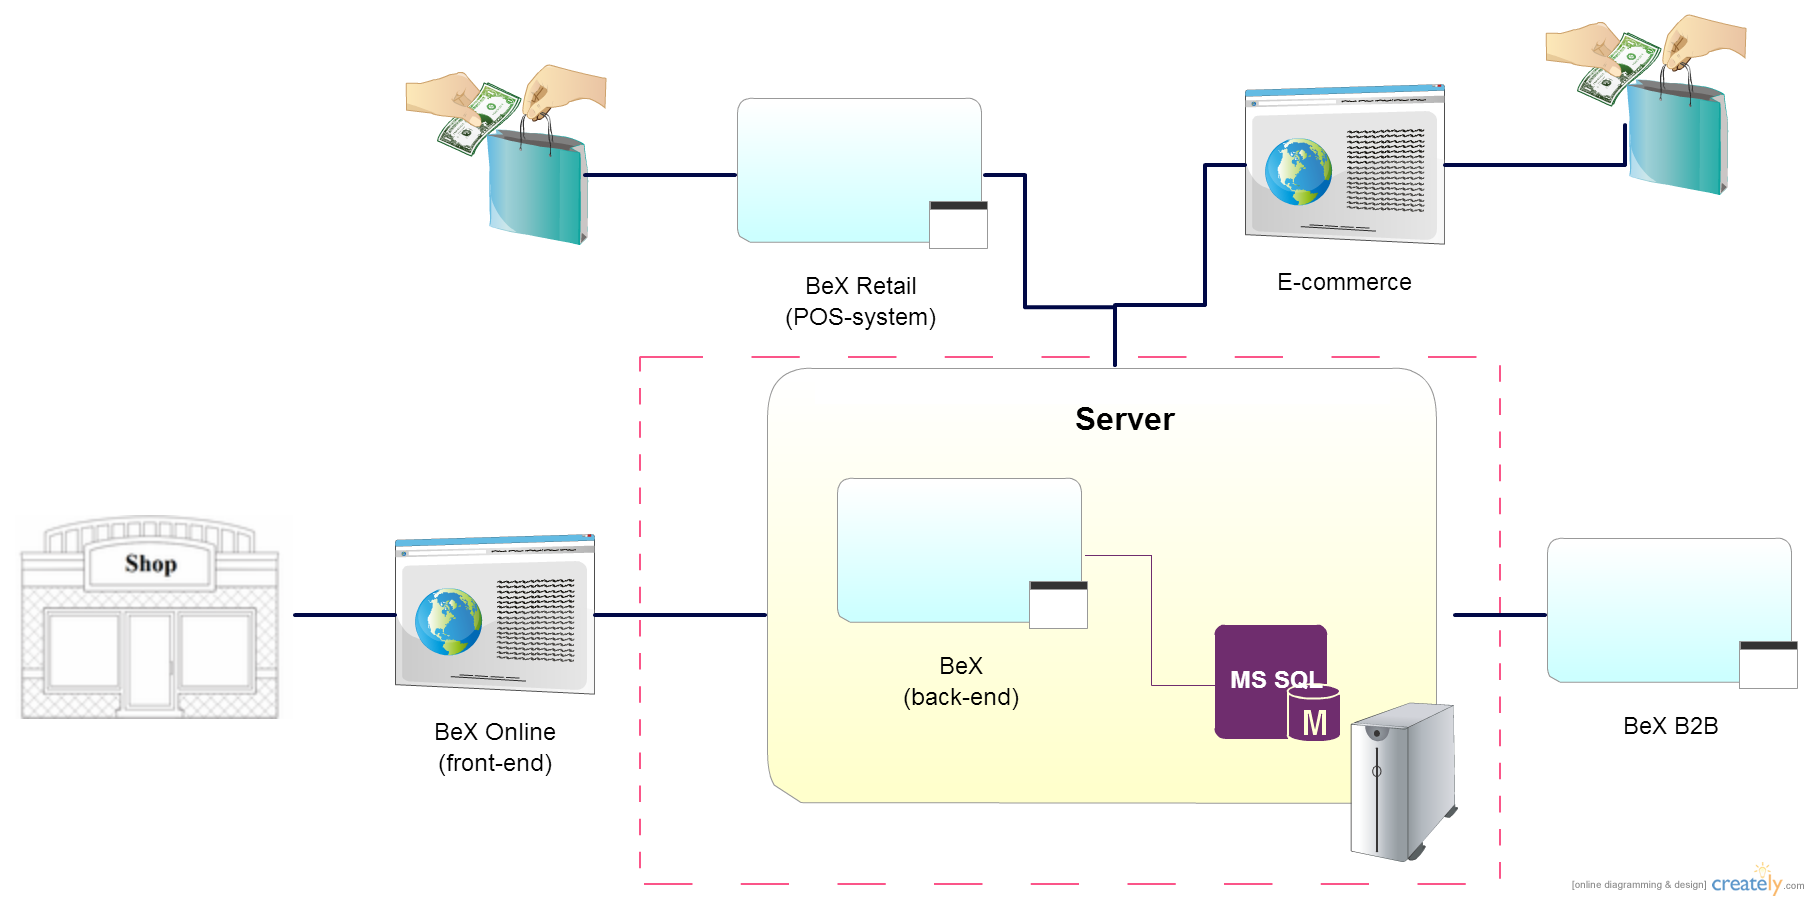
\includegraphics[scale=0.3]{Systemdesc.png}
  \end{center}
  \caption{Context diagram of Perfect IT's system}
  \label{context}
  \vspace{-15pt}
\end{figure}
\noindent The dashed section in Figure~\ref{context} are the components that are of the most interest for this thesis and will be more thoroughly described than the other system components.

\subsection{Components}


\subsubsection{Server}
Microsoft SQL Server Web edition, 64GB Ram, Maximum data capacity: 524 PB, Maximum CPU capacity< 4 socket or 16 cores 

\subsubsection{\bex Online}
\bex Online is a web based system and has a front-end built with HTML5, CSS and JavaScript and a back-end written in C\# and .net with webforms.
Every client have their own instance of the system \todo{deeper description}

\subsubsection{Database}
The database is an essential part of Perfect IT's system and this thesis. All clients share the same physical database but have a unique instance of the database with only their data.  Perfect IT has has to today \hilight{40} clients connected to the servers database, all with different sizes of data ranging from approximately \hilight{5GB data to approximately 60GB} data. The database is an RDBMS and is run on an Microsoft SQL Server 2014 using OLTP and has a total of approximately \hilight{350GB} of data. The database design is largely the same for all the clients, with only a few exceptions among the clients.\\\\ 

\paragraph*{Tables}\mbox{}\\\\
This thesis will be using, until today, the biggest clients database measured in data. To ensure the clients privacy, all sensitive data has been encrypted by the system administrator. \\The default schema is called \textit{dbo} and consists of a total of 254 tables, including some views for big data queries. Many tables are large, considering the amount of rows, where the largest consists of approximately 10.5$\times 10^6$ rows and 80 columns. This table treats the data associated with every transaction made with the client from the start of using this system. There are also empty tables, \hilight{usage?}, that \ldots. The tables form a complex relation to each other and the references are many (as seen in this \href{https://drive.google.com/file/d/0B1IYTmE2hnD-eGQ0N2tvYXZNNVE/view?usp=sharing}{\textcolor{blue}{link}}). In the visualized database reference schema there are tables not referencing any tables at all, \hilight{why?}.\\\\Data obtained from third party applications and API's are also stored in the database and can be seen in the bottom part of the visualized database reference schema mentioned above (\hilight{maybe the answer to the no reference question above?}). Some, \hilight{why not all?} of the BI reports have their own tables in the database, \hilight{why?}.

\paragraph*{Stored procedures}\mbox{}\\\\ 
Stored procedures are subroutines that are available to applications that access relational database systems. Stored procedures are used as centralized logic and can therefore be used by all applications that share the system. These subroutines can include both SQL statements and host language statements, meaning that it can exist of external procedures that has nothing to do with SQL. Often extensive and complex SQL queries, that require a lot of processing and are often being used, are moved to stored procedures for reuse \cite{StoredProcedures}. It's important to know that Stored procedures both bring advantages, e.g. Stored procedures are cached, and drawbacks, e.g. Stored procedure code is not as robust as app code. Subroutines such as Stored procedures should therefore only be used when and if the implementer possess a deep knowledge of the system that is to be affected. It's for example bad practice to store all procedures as Stored procedures for the benefit of the cach-utilization.\\\\
The database in this thesis had a total of 59 Stored procedures treating repetitive procedures by the database mainly for the sales part of the system and the BI reports (there's also a subroutine for locking crucial information, with respect to concurrent execution). These subroutines do not contain any host language statements and/or external procures, but only consists of complex SQL statements. They are present in the system, as mentioned above, to make the execution and processing less demanding, as they are often run by the clients of the system.
 
\section{Theory}
In order to understand why a database might not perform optimally, the following theory was used.

\subsection{Index Fragmentation}
Index fragmentation is one of the most common problems in a relational database. Two kinds of fragmentation can occur, internal index fragmentation and external index fragmentation. The easiest way to explain index fragmentation is by imagining the SQL database as a phone book. At the very end of the book you have a few pages containing a table with indexes of all the entries sorted by last name. This is fine in a static environment such as a phone book but what happens in a dynamic environment?
Since people can be added to the phone book there must be space available after each column in the index, as well as in the pages in the phone book. This is called the \emph{fill factor}. A page can still run out of space and when this happens SQL Server has to add a new page, but it it can't add it at the correct place because the book is already bound. So, it adds blank pages at the very end. This causes two problems, pages with a lot of unused space and pages that are out of order. The first problem is what is referred to as \emph{Internal Fragmentation} and the second is \emph{External Fragmentation}. Internal fragmentation will of course also occur when deleting entries since that leaves "blank space" on the page.\cite{Ozar12}

\subsubsection{Why is this bad for performance?}
At first, internal fragmentation might seem like a good thing. If the phone book has a lot of blank space on every page to start with, adding entries would be super easy and there would be no need for adding more pages later, causing external fragmentation. This is true, but when the number of extra pages needed in the phone book to allow for a lot of blank space is considered, the inefficiency of it becomes apparent. Going through a 100\% filled 1000 page phone book is much faster than a 90\% full 1100 page phone book. So in this example, every time SQL Server needs to scan the index, it would take 10\% longer. Another problem is that the lowest unit for caching in SQL Server is not a record, but a single page, which means that all the empty space must be cached as well. \\

External fragmentation often makes reading the database non-sequential, i.e it cannot be read in order but must be read in random order. This is especially bad in classic magnetic hard drives where the reader head must move around to multiple locations on the drive. Some magnetic hard drives only get 1\% of their sequential reading speed when performing random reads. \cite{Toshiba12}

\subsubsection{Measuring fragmentation}
In Al-Farooque Shubho's article "Top 10 ways to optimize data access in SQL Server"\cite{Shubho09} he explains how to measure if index fragmentation has occurred. By executing the script on page \pageref{lst:fragalg} in Algorithm \ref{See DB-Fragmentation}, index fragmentation is analyzed on every table in the database and presented in a table with an internal and external fragmentation value. \\

According to Shubho, only tables with an internal fragmentation value of less than 75 and/or an external fragmentation value of more than 10 should be considered as fragmented, which this code takes into account.

\subsubsection{Reorganize vs. Rebuild}\mbox{}\\
Both rebuilding and reorganizing are built-in operations in SQL-Server 2014. These are two different operations that both reduce the fragmentation of the indexes. Reorganizing is the more lightweight of the two operations. It fixes the indexes as well as physical reordering of pages and applies any previously set fill factors. Rebuilding builds up a completely new structure for the index. It also allows for a new fill factor.\\
The advantage with reorganizing over rebuilding is that it can be aborted midway, while a rebuild must roll-back after an abort. Usually, in most SQL-systems, a rebuild can't be done while the SQL-server is online. This can be done in MS SQL Server Enterprise edition \cite{Little13}.

\subsubsection{Is it always a good idea to fix fragmentation?}
According to Brent Ozar \cite{Ozar12} fixing fragmentation can cause more damage than keeping fragmented indexes. Often administrators try to fix fragmentation by using a low fill factor, say 50\%. This would mean that half of every page would be blank, which would make writing really fast. Reading however, would be twice as slow. Another common mistake is to rebuild every single index in the database, even though some tables might not had a single write since the last time. This is a problem because defragmenting indexes causes SQL Server to write to the transaction log. The bigger a log is, the longer log backups and restores take.\\\\
Another important factor is that external fragmentation mostly causes problems when the database is stored in disc, since classical hard drives are slow at random reading. If the database is instead stored in memory, which is almost as fast at random reading as sequential reading, external fragmentation won't be as big a issue.

\subsection{Query Tuning}

\subsection{In-Memory Database}
Relational database management systems were originally designed in the late 70's\cite{Nevarez}. Because of this, they are designed with the assumption that memory is limited, expensive and that the size of the database is many times larger than the main memory. This is not longer true. Memory (RAM) is relatively cheap and it's possible to have 100s of GB of RAM in a single server. In Vizard's article\cite{Vizard12} it is said that having a database system completely in memory could make an application a thousand time faster.


\section{Analysis}

\subsection{Index fragmentation}
By using the script from the theory the following index fragmentation values were produced. The table names and index names has been changed due to confidentiality.

\begin{table}[H]
\begin{center}
\begin{tabular}{|l|l|l|l|}
\hline
Table name & Index name & External fragmentation & Internal fragmentation \\ \hline 
1  & a & 100         & 74,05485545 \\ \hline
2  & b & 100         & 72,6278725  \\ \hline
3  & c & 100         & 58,68544601 \\ \hline
4  & d & 100         & 70,17500618 \\ \hline
5  & e & 100         & 67,92068199 \\ \hline
6  & f & 100         & 58,46971831 \\ \hline
7  & g & 100         & 50,03706449 \\ \hline
8  & h & 99,48535234 & 57,89085743 \\ \hline
9  & i & 96,11111111 & 73,69038794 \\ \hline
10 & j & 94,44444444 & 70,63737336 \\ \hline
11 & k & 90,59325223 & 52,81183593 \\ \hline
12 & l & 89,13043478 & 65,47550037 \\ \hline
13 & m & 86,99186992 & 65,83502595 \\ \hline
14 & n & 85,71428571 & 47,9579318  \\ \hline
15 & o & 78,98550725 & 57,05273042 \\ \hline
16 & p & 77,77777778 & 56,54531752 \\ \hline
17 & q & 75          & 48,44946874 \\ \hline
18 & r & 73,35790885 & 62,85373116 \\ \hline
19 & j & 71,30559541 & 64,10468248 \\ \hline
20 & s & 69,67213115 & 69,75221151 \\ \hline
21 & m & 68,46173667 & 65,69195701 \\ \hline
22 & t & 67,79506955 & 65,90287868 \\ \hline
23 & u & 66,66666667 & 49,09809736 \\ \hline
24 & v & 50          & 74,49962936 \\ \hline
25 & w & 50          & 53,43464295 \\ \hline
26 & x & 50          & 54,92957746 \\ \hline
27 & y & 50          & 41,83552014 \\ \hline
28 & z & 36,59652333 & 72,06630838 \\ \hline
29 & å & 33,5729147  & 73,20072894 \\ \hline
\end{tabular}
\caption{Results from index fragmentation search}
\end{center}
\end{table}

This shows that a some of the indexes used have well over an external fragmentation value of 10. The internal fragmentation value is also bad at some of the indexes (i.e less than 75).

\chapter{Proposed Solution}\label{sec:proposedsoluton}

\section{Solution Introduction}

\section{Integration}

\chapter{Software Development \& Testing}

\chapter{Discussion}

\chapter{Conclusions}
\addcontentsline{toc}{chapter}{Bibliography}
\bibliographystyle{plain}

\bibliography{MyMSc}

\begin{appendices}

\chapter{Code}
\begin{lstlisting}[caption={Algorithm to find fragmented tables and the fragmentation values.},label=See DB-Fragmentation]
SELECT object_name(dt.object_id) Tablename,si.name
IndexName,dt.avg_fragmentation_in_percent AS
ExternalFragmentation,dt.avg_page_space_used_in_percent AS
InternalFragmentation
FROM
(
    SELECT object_id,index_id,avg_fragmentation_in_percent,avg_page_space_used_in_percent
    FROM sys.dm_db_index_physical_stats (db_id('AdventureWorks'),null,null,null,'DETAILED'
)
WHERE index_id <> 0) AS dt INNER JOIN sys.indexes si ON si.object_id=dt.object_id
AND si.index_id=dt.index_id AND dt.avg_fragmentation_in_percent>10
AND dt.avg_page_space_used_in_percent<75 ORDER BY avg_fragmentation_in_percent DESC
\end{lstlisting}
\label{lst:fragalg}
\end{appendices}
\end{document}